% grundlagen/octree.tex
%Octree als Schnittstelle zwischen CAD und Simulation (Vor-Nachteile, 
%Datenstruktur)
%
% Ausarbeitung zur Diplomarbeit Nr. 2035 - "Erzeugung und Evaluierung 
% von Oktalbaumstrukturen als Schnittstelle zu CAD-Programmen"
%
% Autor: Stefan Mahler 2002
%   Universitaet Stuttgart, SgS
% Betreuer: Ralf Mundani

\section{Der Oktalbaum als Schnittstelle zwischen CAD und Simulation}
\label{schnittstelle_octree}
Bei Simulationen besitzt die Lokalisation innerhalb eines geometrischen 
Modells -- also die Bestimmung, wo sich ein Punkt bzw. eine Zelle bez"uglich 
eines K"orpers befindet -- einen hohen Stellenwert. 
Sie muss deshalb durch das Modell effizient erfolgen k"onnen. 
Aus diesem Grund sind f"ur Simulationsaufgaben nur direkte 
Volumenmodelle vorteilhaft. Dabei sollte die bei Simulationen auftretenden 
Raumdiskretisierungen durch das Modell unterst"utzt werden. Dem 
Oktalbaumschema kommt dabei eine hohe Bedeutung zu, da es eine Reihe von 
Vorteilen gegen"uber anderen Modellen hat. Das f"allt besonders gegen"uber 
dem ebenfalls in diesem Zusammenhang bedeutenden Normzellen-Aufz"ahlungsschema 
auf. Ursache hierf"ur sind vor allem die im Oktalbaumschema vorkommenden 
Organisationsprinzipien.
 
W"ahrend beim Normzellen-Aufz"ahlungsschema "uber 
das gesamte Gebiet die Zellen die gleiche (minimale) Gr"o"se besitzen, wird 
beim Oktalbaumschema nur der Rand des K"orpers maximal aufgel"ost. Verdoppelt 
man die Aufl"osung in jede Raumrichtung, ist nicht -- wie beim 
Normzellen-Aufz"ahlungsschema -- mit einer achtfach, sondern nur mit einer 
vierfach h"oheren Gesamtzellzahl zu rechnen. 
Da Zeit- und Speicheraufwand von der Gesamtzellanzahl abh"angen, gelten 
f"ur sie equivalente Komplexit"atsabsch"atzungen. Ist bereits ein Oktalbaum 
geringerer Aufl"osung vorhanden, m"ussen nur die Randknoten (ausgehend von 
der gr"oberen Aufl"osung) verfeinert und nicht 
der ganze Oktalbaum neu erzeugt 
werden, was weitere Geschwindigkeitsvorteile 
bringt. 
Auf Oktalb"aumen lassen sich Normzellen-Aufz"ahlungsschemata 
'emulieren', 
womit der Oktalbaum prinzipiell auch "uberall dort eingesetzt 
werden kann, wo ein Normzellen-Aufz"ahlungsschema verwendet wird. 
Ein weiteres Indiz f"ur die Vorteile der Verwendung des Oktalbaums als 
Schnittstelle ist seine Verwendung in unterschiedlichsten 
Anwendundungsgebieten, da dies f"ur seine flexible Nutzbarkeit spricht. 

\subsection{Anwendungsgebiete f"ur Oktalb"aume}
Neben der Simulation kommen Oktalb"aume in anderen wichtigen Gebieten zum 
Einsatz. Hierzu nennt \cite[S. 26]{diss_oct} 
\begin{itemize}
\item die Bildverarbeitung: zur Erzeugung eines 3D-Modells aus 2D-Daten (z.B. 
    CT-Daten), zur effizienten Bilddatenspeicherung und -reduktion, zum
    Einf"arben von Fl"achen oder zur Bild- oder Objekterkennung,
\item die Computergrafik: zur Sichtbarkeitsentscheidung oder 
    R"uckseitenerkennung, sowie in den Bereichen Raytracing, Radiosity oder 
    Animation,
\item die Visualisierung: zur Isofl"achengenerierung beim Volume Rendering 
    und
\item die Robotik: zur Interferenzdetektion oder Bahnplanung.
\end{itemize}

Wird die Oktalbaumstruktur zur Gittergenerierung f"ur Simulationsaufgaben 
verwendet, dient sie meist als n"utzliches Hilfskonstrukt, die vor der 
eigentlichen Simulation nachbearbeitet werden muss.

\subsection{Datenstrukturen f"ur Oktalb"aume}
Aus der Definition von Oktalb"aumen (vgl. Abschnitt \emph{Oktalb"aume} 
\vpageref{einf_octree}) 
ergibt sich die Verwendung von hierachisch rekursiven Datenstrukturen f"ur 
Oktalb"aume. 
Folgende Beziehungen sind dabei wichtig (unter '\opitemlabel' sind m"ogliche 
Operationen\footnote{Dies sind die Methoden, die in dieser Arbeit hierf"ur 
werden.} 
dargestellt, mit denen der Status dieser Beziehungen ermittelt werden kann. 
Diese Operationen, sowie analoge Operationen zur Modifikation 
m"ussen die entsprechenden Datenstrukturen bereitstellen):
\begin{itemize}
\item Durch Knoten werden begrenzte Volumina wiedergegeben. 
\item Es gibt einen ausgezeichneten Knoten, die \emph{Wurzel}. Er 
    repr"asentiert den \emph{boundary cube} -- also ein die gesamte 
    modellierte Geometrie einh"ullender W"urfel. Die Wurzel ist 
    Einstiegsknoten 
f"ur den Oktalbaum, "uber sie k"onnen alle anderen Knoten 
    erreicht werden. Jeder Knoten kann "uber genau einen Weg von der Wurzel 
    aus erreicht werden.
    \oplistbeg
    \label{basis_op_beg}
    \opitem \funcdef{getRoot}{}{\_octree} liefert die Wurzel.
    \oplistend
\item "Uber die Verfeinerungsaktion bei der Oktalbaumgenerierung entstehen 
    Unteroktanten zu einem bestimmten Volumen, woraus sich eine  
    Hierachie ergibt. Die Wurzel stellt die 
    h"ochste Hierachieebene dar. Die Knoten, die die Untervolumina 
    repr"asentieren, die durch eine Verfeinerungsaktion hervorgegangen sind, 
    werden als Sohnknoten zu einem Vaterknoten bezeichnet. Die Wurzel ist  
    der einzigste Knoten ohne Vaterknoten, alle anderen Knoten besitzen genau 
    einen Vaterknoten.
\item Entsprechend der Verfeinerungstiefe ergibt sich somit eine Knotentiefe 
    $d$ f"ur einem Knoten innerhalb des Baums. Der Wurzel wird die Tiefe $0$ 
    zugewiesen. Sohnknoten $c$ haben eine um $1$ gr"o"sere Tiefe als ihr 
    Vaterknoten $p$: $d_c = d_p + 1$.
    Als Tiefe $d_t$ des Baums $t$ ergibt sich die maximale Tiefe eines 
    Knoten $n$ des Baums: $d_t = \max_{n \in t} \{ d_n \}$. 

    Es kann eine maximale Verfeinerungstiefe definert definiert werden.  
    Damit ergibt sich auch eine \emph{maximale Baumtiefe} $d_{t_{\max}}$. 

    Manchmal ist es g"unstiger die \emph{Knotenh"ohe} $h_n$ anstatt seiner 
    Tiefe festzulegen. Ein Oktalbaumknoten auf der untersten Verfeinerungstiefe
    ($d_n = d_{t_{\max}}$) hat die H"ohe $h_n = 0$. Er muss immer ein Blatt 
    sein.
    Der Wurzelknoten besitzt die H"ohe $d_{t_{\max}}$. Sohnknoten $c$ haben 
    eine um $1$ niedrigere H"ohe als ihr Vaterknoten $p$: $h_c = h_p - 1$.
    Zwischen Knotentiefe und Knotenh"ohe besteht folgender Zusammenhang: 
    \hbox{\(h_n = d_{t_{\max}} - d_n\)}.
    \oplistbeg
    \opitem \funcdef{getMaxTreeDepth}{}{Depth} liefert die maximale 
	Baumtiefe $d_{t_{\max}}$.
    \oplistend
    
    Des Weiteren besteht zwischen Knotentiefe $d_n$ und der L"ange des 
    von ihm repr"asentierten W"urfels $l_n$ folgender Zumsammenhang:
    \gl{gl_knotentiefe_zellgroesse}{l_n = \frac{l_0}{2^{d_n}}\mbox{.}}
    $l_0$ ist die L"ange der boundary cube bzw. des modellierten 
    Gesamtvolumens, was durch den Oktalbaum repr"asentiert wird. Dieser 
    Zusammenhang wird noch sp"ater zur Indizierung von Oktalbaumknoten 
    und zur Zuordnung von Punkten zu einer Zelle des Oktalbaums verwendet. 
\item Ist ein Knoten Vaterknoten, besitzt er also Sohnknoten, wird er als 
    \emph{innerer Knoten} bezeichnet. Aus der Definition des Oktalbaums ergibt 
    sich, dass jeder innere Knoten genau acht S"ohne besitzt. Dabei sind 
    die Oktanten (und damit die acht S"ohne) in einer bestimmten Reihenfolge 
    festgelegt.
    Die restlichen Baumknoten sind \emph{Bl"atter}, die demzufolge keine 
    S"ohne besitzen. Bl"atter von Oktalb"aumen besitzen ein wichtiges 
    Attribut, welches definiert, ob der dadurch repr"asentierte Raumteil zu 
    einem K"orper geh"orig (in) oder nicht (out) oder auf dem Rand des 
    K"orpers 
    befindlich (on) zu z"ahlen ist. In dieser Arbeit wurde jedoch dieses 
    Attribut auf Grund der folgenden Anforderungen etwas abweichend 
    definiert: 
    \begin{itemize}
    \item Der Rand soll immer zu dem K"orper 
geh"orig gez"ahlt werden. 
    \item Mehrere K"orper k"onnen durch einen 
Oktalbaum modelliert werden. 
    \end{itemize}
    Das Attribut speichert hier eine Farbe. 
    Jedem K"orper wird eine Farbe eineindeutig zugeordnet. Eine weitere 
    Farbe ist als \emph{zu keinem K"orper geh"orend} defniert. Alle Bl"atter 
    die Raumteile repr"asentieren, die zu keinem K"orper geh"oren, werden mit 
    dieser speziellen Farbe markiert.
    \oplistbeg
    \opitem \funcdef{isLeaf}{Node node}{\bool} liefert \true{} falls 
	\param{node} ein Blatt ist und f"ur innere Knoten \false.
    \opitem \pre{\func{isLeaf}{node} $=$ \false{}, \param{i} $\in [0, 7]$}\\
	\funcdef{getChild}{\_octree parent, Parttype i}{\_octree} liefert 
	den \param{i}-ten Sohn zum Vaterknoten \param{parent}.
    \opitem \pre{\func{isLeaf}{node} $=$ \true{}}\\
	\funcdef{getColor}{Node node}{Color} liefert die Farbe des Blatts.
    \opitem \pre{\func{isLeaf}{node} $=$ \true{}}\\
	\funcdef{isNoObject}{Node node}{\bool} liefert \true{} falls 
	\func{getColor}{node} $=$ \emph{'zu keinem K"orper geh"orend'} und 
	sonst \false{}.
    \oplistend
\end{itemize}
Hiermit sind wesentliche Beziehungen, die f"ur Oktalb"aume gelten, definiert. 
B"aume im Allgemeinen besitzen eine Reihe von weiteren interessanten 
Eigenschaften, welche u.a. in \cite{algo_cpp} beschrieben sind.

Im Weiteren werden vier Datenstrukturen vorgestellt, die f"ur 
Oktalbaumstrukturen eingesetzt werden. Besondere Bedeutung innerhalb dieser 
Arbeit haben das \emph{baumartige Zeigergeflecht} und die 
\emph{Pr"aorder-Traversierung}. Das baumartige Zeigergeflecht ist Basis f"ur 
die Oktalbaumstruktur, die zur Generierung des Oktalbaummodells benutzt wurde
(vgl. Kapitel \ref{algo}). Hierauf wurde ein Index analog zur 
\emph{Positionscodierung} definert.
Zum permanenten Datenhaltung wurde das Zeigergeflecht mit Hilfe der 
Pr"aorder-Traversierung linearisiert (vgl. Abschnitt \ref{export_pot}).

\subsubsection{Baumartiges Zeigergeflecht}
Das Zeigerflecht wird h"aufig zur Veranschaulichung von B"aumen verwendet und 
ist daher die naheliegendste Datenstruktur. Sie besitzt folgende wesentliche 
Eigenschaften:
\begin{itemize}
\item Auf jedes Blatt kann in $\mathcal{O}(d)$ Zeit zugegriffen werden. 
    Dabei ist $d$ die Blatttiefe. Oktalb"aume besitzen in typischen 
    Anwendungen eine Tiefe von $6$ bis $15$.
\item Da es sich bei einem Zeigergeflecht um eine dynamische Struktur handelt, 
    ist sie leicht anpassbar. Modifikationen k"onnen effizient durchgef"uhrt 
    werden. So wird z.B. f"ur das Einf"ugen oder L"oschen von Bl"attern 
    $\mathcal{O}(d)$ Zeit ben"otigt. Es gibt keine strukturbedingten 
    Gr"o"senbeschr"ankungen, wie z.B. bei statischen Feldern. Auch k"onnen 
    Hilfszeiger eingef"ugt werden. So kann z.B. der Nachbar eines Blatts 
    in $\mathcal{O}(1)$ gefunden werden, wenn entsprechende Referenzen zuvor 
    im Oktalbaum gesetzt wurden. Durch das Einf"ugen von zus"atzlichen 
    Zeigern ergeben sich nat"urlich auch Nachteile, wie z.B. zus"atzlicher 
    Aufwand f"ur die Konsistenzhaltung das Oktalbaums.
\item Je nach Speicherarchitektur werden zus"atzlich f"ur jeden Zeiger 
    $1$ bis $2$ W"orter zum Speichern dieses Zeigers ben"otigt. Das ist 
    meist sogar mehr, als an Speicherplatz f"ur die eigentliche Information 
    (Blatt oder kein Blatt, Blattfarbe) verbraucht wird. Zeigergeflechte 
    verbrauchen deshalb gerade bei gr"o"seren Strukturen mehr Speicher 
    als kompakte Datenstrukturen.
\item Allgemein bedingt die Benutzung von Zeigern insbesondere bei starken 
    Modifikationen (st"andiges Einf"ugen und L"oschen von Knoten) einige 
    technische Probleme. Zum Beispiel 
    \begin{itemize}
    \item k"onnen mehrere Zeiger gleiche Knoten referenzieren (im Oktalbaum: 
	wenn er durch zus"atzliche Referenzen beispielsweise auf die 
	Nachbarknoten erweitert wird). Wird der entsprechende 
	Speicherbereich "uber den einen Zeiger freigegeben, enth"alt der 
	andere Zeiger eine falsche Referenz.
    \item muss das Problem des \emph{Carbage Collection} beachtet werden. 
	Es muss eine Instanz geben, die sich um nicht mehr verwendete  
	Speicherbereiche k"ummert. Es k"onnen Segmentierungen des 
	Haldenspeichers auftreten. Es ist zu beachten, dass Speicherbereiche, 
	die nicht mehr verwendet und dennoch nicht freigegeben werden~--, wie 
	z.B. bei Ringlisten, auftreten k"onnen.
	Der Cabage Collector kann zeitliche Abl"aufe des Programms 
	beeinflussen und die Laufzeiteigenschaften des Programms 
	verschlechtern.  
    \end{itemize}
\end{itemize}

Abbildung \ref{abb_quad_ref} zeigt das Zeigergeflecht zum Quadtree in 
Abbildung \ref{abb_pos_quad}.

\diabeg
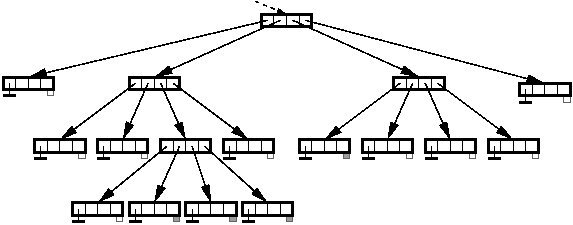
\includegraphics[scale=0.5]{quad_ref}
\caption{Zeigergeflecht eines Quadtree}
\label{abb_quad_ref}
\diaend

\subsubsection{Positionscodierung}
\label{pos_code}
Bei der Positionscodierung erh"alt jeder Knoten einen eindeutigen Index. 
F"ur die Sohnknoten muss eine bestimmte Reihenfolge definiert werden, woraus 
sich ein entsprechendes Nummerierungsschema ableitet.
H"aufig wird die Reihenfolge an Hand der Lebesgue-Kurve festgelegt. 
Der Index eines Knotens ist dann der Vektor, der sich aus Nummern der Knoten 
ergibt, die auf dem Pfad von der Wurzel zu ihm besucht wurden. 
Besonders anschaulich ist die Verwendung von Oktalzahlen f"ur den Index. 
Jede Ziffer gibt die Nummer des entsprechenden Sohnknotens wieder. Die Anzahl 
der Ziffern liefert die Tiefe des indizierten Knotens. Hiermit kann auch 
die Position der Zelle des Oktalbaums bestimmt werden, die dem Knoten 
zugeordnet ist. Hierher r"uhrt auch der Name Positionscodierung f"ur diese 
Repr"asentationsform. Abbildung \ref{abb_pos_quad}a) zeigt die 
Positionscodierung nach diesem Verfahren im 2-Dimensionalen zu einem Quadtree. 

Gegen"uber dem Zeigergeflecht ist die Identifikation von Knoten einfacher, 
woraus eine Vereinfachung verschiedener Algorithmen resultiert. 

In dieser Arbeit wird eine leicht abgewandelte Form benutzt, die besonders 
intuitiv ist und auf der das Normzellenschema leicht simuliert werden kann.
Es wird jede Raumrichtung gesondert betrachtet, wodurch ein 3-dimensionaler 
Vektor aus Bin"arzahlen entsteht. Somit wird f"ur jede Raumrichtung bestimmt, 
ob der Sohn im jeweils vorderen oder hinteren Teilraum liegt. 
Zus"atzlich wird noch die Knotenh"ohe im Index vermerkt (vgl. Abbildung 
\ref{abb_pos_quad}b). 

\diabeg[!t]
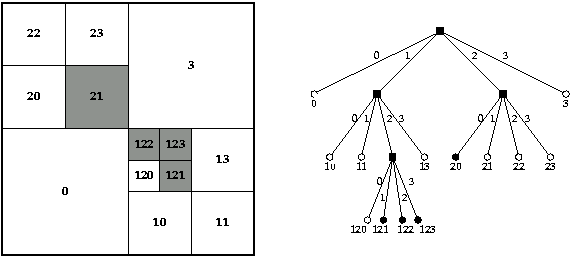
\includegraphics[scale=.75]{pos_quad_classic}
\begin{center}
\emph{a) "ublich}
\end{center}
\vspace{1.5em}
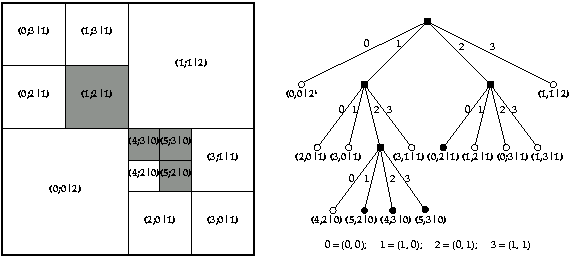
\includegraphics[scale=.75]{pos_quad_alt}
\begin{center}
\emph{b) in dieser Arbeit verwendet}
\end{center}
\caption{Positionscodierung}
\label{abb_pos_quad}
\diaend

Die Positionscodierung wird in der Literatur auch als \emph{linearer Code} 
oder \emph{leafcode} bezeichnet. 


\subsubsection{Codierung "uber Raum-Position und Gr"o"se}
Statt "uber den Pfad durch den Baum l"asst sich ein Knoten auch "uber seine 
Position $P$ im Raum und seine Gr"o"se $G$ identifizieren. Die Position 
kann dabei "uber die Koordinaten eines bestimmten Zellpunkts, "uber die Anzahl 
der Maschenweiten eines virtuellen Gitters feinster Aufl"osung oder durch 
eine Bin"aradresse "ahnlich der Positionscodierung dargestellt werden. 
Die Gr"o"se wird entweder durch die reale Gr"o"se oder ein Vielfaches der 
Maschenweite angegeben. 
Nachteilig an dieser Repr"asentationsform ist die fehlende Unterst"utzung des 
Organisationsprinzips Hierachie.

Der in Abbildung \ref{abb_pos_quad} dargestellte Quadtree k"onnte durch 
folgenden Code~$C=(P;G)$ dargestellt werden: 

\begin{tabularx}{\linewidth}{lX}
Bl"atter: & (0,~0;~4), (0,~4;~2), (0,~6;~2), (2,~4;~2), (2,~6;~2), (4,~0;~2), 
	    (4,~2; 1), (4,~3;~1), (4,~4;~4), (5,~2;~1), (5,~3;~1), (6,~0;~2), 
	    (6,~2;~2)\\
inner Knoten: & (0,~0;~8), (0,~4;~4), (4,~0;~4), (4,~2;~2)
\end{tabularx}

\subsubsection{Pr"aorder-Traversierung}
\label{pot_code}
Es gibt unterschiedliche Formen, um alle Knoten eines Baums abzulaufen, also 
zu traversieren. Durch Tiefensuche "uber den Baum entsteht, je nachdem ob 
dabei der Vaterknoten vor, in der Mitte oder nach den S"ohnen notiert wird, 
\emph{Pr"aorder-}, \emph{Inorder-} oder \emph{Postorder-Traversierung}. 
Wird Breitensuche angewendet, also alle Knoten einer Tiefe besucht, 
bevor ihre S"ohne besucht werden, entsteht eine 
\emph{Levelorder-Traversierung}.

F"ur Oktalb"aume wird dabei h"aufig die Pr"aorder-Traversierung verwendet. 
Da innere Knoten stets acht S"ohne besitzen, ist eine besonders kompakte 
Darstellung m"oglich: Beispielsweise k"onnen innere Knoten mit {\tt 1}, 
Bl"atter 
mit {\tt 0} markiert werden. 
Das zus"atzliche Farbattribut wird einfach hinter die blattmarkierende {\tt 0} 
hinzugef"ugt. Damit liegt der Oktalbaum sehr kompakt in einer linearisierten 
Form vor und kann somit als bin"arer Strom (binary Stream) verarbeitet werden. 

Mit dieser Codierung ergibt sich f"ur den Quadtree aus Abbildung 
\ref{abb_pos_quad}:
\begin{alltt}
1001000 01000101 01001010 0000000
\end{alltt}

Die Pr"aorder-Traversierung wird auch Depth-First-Strategie genannt. In der 
Literatur kommen auch die Namen \emph{DF-expression} oder \emph{treecode} f"ur 
diese Form der Codierung vor.

\subsection{Operationen auf Oktalb"aumen}
Neben den im Abschnitt \ref{basis_op_beg} beschriebenen grundlegenden 
Operationen, gibt es weitere Grundoperationen auf einem Oktalbaum.
Hierzu geh"oren das Erzeugen, L"oschen oder die Aufspaltung eines Blatts, 
sowie die Vereinigung gleichgef"arbter Bl"atter zu einem Blatt der 
dar"uberliegenden Ebene (Kompaktieren). Diese Operationen sind auf den hier 
verwendeten Zeigergeflecht als Basisstruktur leicht effizient zu realisieren. 

Raumpartitionierende Strukturen -- und somit der Oktalbaum -- sind geradezu 
pr"adestiniert f"ur die bin"aren Mengenoperationen Schnitt, Vereinigung 
und Differenz: Die beiden B"aume werden synchron (z.B. durch 
Pr"aorder-Traversierung) durchlaufen und an den Bl"attern entsprechende 
Vergleiche durchgef"uhrt, um so den resultierenden Baum zu konstruieren. 
In der Literatur finden sich auch effiziente Algorithmen zur Realisierung der 
affinen Transformationen Translation, Rotation und Skalierung. 

Des Weiteren ist die Bestimmung der Nachbarzelle zu einem Oktalbaumknoten 
von Bedeutung. 
Die Nachbarzelle ist jedoch nicht direkt aus der Oktalbaumstruktur ersichtlich, 
insbesondere wenn diese durch ein Zeigergeflecht repr"asentiert wird. Hierf"ur 
wird die Positionscodierung verwendet. Mit dem in dieser Arbeit verwendeten 
Index (vgl. Abschnitt \emph{Positionscodierung} \vpageref{pos_code}) kann 
leicht der entsprechende 'theoretische' Nachbar auf gleicher Ebene ermittelt 
werden. Der so ermittelte Nachbar kann jedoch unterhalb des 'realen' Nachbars 
liegen, wenn der entsprechende Baumast nicht so tief ist wie der 
Ausgangsknoten. 
Mit Hilfe von \funcdef{getExistNode}{NodeIndex p}{NodeIndex} 
(\algref{alg_getexistnode_idx}) wird deshalb der Index des tiefsten 
existierenden Knotens ermittelt, der sich auf dem Pfad zu \param{p} befindet. 
Der so gefundene Knoten muss jedoch nicht ein Blatt sein. Diese k"onnen durch 
rekursiven Abstieg zu den entsprechenden S"ohnen (Gegenrichtung als die 
Richtung zum Nachbarn) gefunden werden.

Es finden sich Algorithmen, die einen balancierten Oktalbaum voraussetzen. 
\emph{Balanciert} bedeutet, dass sich die Maschenweite zweier benachbarten 
Zellen um maximal den Faktor $2$ unterscheiden (also die Tiefe von 
Nachbarknoten maximal um $\pm 1$ differiert). 
Da sich Aufspaltungen oder Vereinigungen 
innerhalb einer Zelle bei der Balancierung h"ochstens auf deren 
Nachbarzellen auswirken, haben "Anderungen im Baum nur lokale Wirkung. 
Somit l"asst sich die Balancierung eines Baums effizient umsetzen.

Zur Aufz"ahlung r"aumlich angeordneter diskreter Daten -- entsprechend 
der Lebesgue-Kurve -- kann der \emph{Morton-Index} verwendet werden. 
Als herausragende Eigenschaft ist zu nennen, dass Nachbarschaftsbeziehungen 
in einer so erzeugenden Sequenz bereits im urspr"unglichen Baum vorhanden
waren. 
Der Morton-Index kann so effizient zur Nachbarschaftsbestimmung von Knoten 
im Oktalbaum genutzt werden und eignet sich zur dimensionsunabh"angigen 
Sequentialisierung von Quad-/Octree-Zeigerstrukturen. 
Ferner kann der Morton-Index zur 
Oktalbaumgenerierung aus einem 
Normzellen-Aufz"ahlungsschema verwendet werden.

%% End of Document
